\documentclass[12pt]{article}

% ------------------------------------------------------------------
% Core math
\usepackage{amsmath, amssymb, amsthm}
% Diagrams
\usepackage{tikz-cd}
\usepackage{tikz}
\usetikzlibrary{arrows.meta, positioning, calc, fit, backgrounds}
% Graphics
\usepackage{graphicx}
% Tables
\usepackage{longtable}
\usepackage{array}
\usepackage{booktabs}
% Page layout
\usepackage[margin=1in]{geometry}
% Colour / symbols
\usepackage{xcolor}
\usepackage{mathtools}
\usepackage{stmaryrd}
\usepackage{enumitem}
% References: hyperref loaded as late as possible; cleveref strictly after it.
\usepackage{hyperref}
\usepackage{cleveref}

\hypersetup{
  colorlinks=true,
  linkcolor=blue!55!black,
  citecolor=green!45!black,
  urlcolor=blue!55!black,
  pdftitle={A Modular Representation Synthesis: Composing Six Mathematical Faculties into Physical Representation},
  pdfauthor={Matthew Long}
}

% ------------------------------------------------------------------
% Theorem environments
\newtheorem{theorem}{Theorem}[section]
\newtheorem{proposition}[theorem]{Proposition}
\newtheorem{lemma}[theorem]{Lemma}
\newtheorem{corollary}[theorem]{Corollary}
\theoremstyle{definition}
\newtheorem{definition}[theorem]{Definition}
\newtheorem{axiom}{Axiom}
\newtheorem{example}[theorem]{Example}
\newtheorem{conjecture}[theorem]{Conjecture}
\theoremstyle{remark}
\newtheorem{remark}[theorem]{Remark}
\newtheorem{principle}[theorem]{Principle}
% cleveref display names for custom counters
\crefname{axiom}{Axiom}{Axioms}
\Crefname{axiom}{Axiom}{Axioms}

% ------------------------------------------------------------------
% Notation macros (aligned with Parts I--VI)
\newcommand{\Dom}{\mathsf{Dom}}
\newcommand{\Math}{\mathsf{Math}}
\newcommand{\Phys}{\mathsf{Phys}}
\newcommand{\Info}{\mathsf{Info}}
\newcommand{\Rep}{\mathsf{Rep}}
\newcommand{\Meas}{\mathsf{Meas}}
\newcommand{\Gpd}{\mathsf{Gpd}}
\newcommand{\Grpd}{\mathbf{Grpd}}
\newcommand{\Cat}{\mathsf{Cat}}
\newcommand{\Set}{\mathsf{Set}}
\newcommand{\Vect}{\mathsf{Vect}}
\newcommand{\Bord}{\mathsf{Bord}}
\newcommand{\Real}{\mathrm{Real}}
\newcommand{\Obs}{\mathrm{Obs}}
\newcommand{\Repphys}{\mathsf{Rep}_{\mathrm{phys}}}
\newcommand{\Aut}{\operatorname{Aut}}
\newcommand{\Stab}{\operatorname{Stab}}
\newcommand{\Hom}{\operatorname{Hom}}
\newcommand{\iHom}{\underline{\operatorname{Hom}}}
\newcommand{\op}{\mathrm{op}}
\newcommand{\per}{\mathrm{per}}
\newcommand{\id}{\mathrm{id}}
\newcommand{\Spec}{\operatorname{Spec}}
\newcommand{\physrep}[1]{\llbracket #1 \rrbracket_{\mathrm{phys}}}
\newcommand{\Sstat}{\textsf{S}}
\newcommand{\Hstat}{\textsf{H}}
\newcommand{\Pstat}{\textsf{P}}
\newcommand{\stle}{\preceq}
\newcommand{\Ho}{\mathcal{H}}
\newcommand{\Hphys}{\Ho_{\mathrm{phys}}}
\newcommand{\Hlog}{\Ho_{\mathrm{log}}}
\newcommand{\Hgauge}{\Ho_{\mathrm{gauge}}}
\newcommand{\Herr}{\Ho_{\mathrm{err}}}
\newcommand{\Amp}{\mathcal{A}}
\newcommand{\Ampm}{\mathcal{A}^{\mathfrak{m}}}
\newcommand{\Lcoalg}{\mathcal{L}}
\newcommand{\Mot}{\mathrm{Mot}}
\newcommand{\ZZ}{\mathbb{Z}}
\newcommand{\CC}{\mathbb{C}}
\newcommand{\QQ}{\mathbb{Q}}
\newcommand{\MtoP}{Math\textrightarrow{}Physics}
% roman-numeral module tags
\newcommand{\PI}{\textsc{i}}
\newcommand{\PII}{\textsc{ii}}
\newcommand{\PIII}{\textsc{iii}}
\newcommand{\PIV}{\textsc{iv}}
\newcommand{\PV}{\textsc{v}}
\newcommand{\PVI}{\textsc{vi}}

% GrokRxiv DOI sidebar (modern shipout hook; page-1 only)
\definecolor{grokgray}{RGB}{110,110,110}
\AddToHook{shipout/background}{%
  \ifnum\value{page}=1
    \begin{tikzpicture}[remember picture, overlay]
      \node[
        rotate=90,
        anchor=south,
        font=\Large\sffamily\bfseries\color{grokgray},
        inner sep=0pt
      ] at ([xshift=38pt, yshift=0.52\paperheight]current page.south west)
      {GrokRxiv:2026.07.synthesis\quad
       [\,math.CT / hep-th\,]\quad
       04 Jul 2026};
    \end{tikzpicture}
  \fi
}

% ------------------------------------------------------------------
\title{\textbf{A Modular Representation Synthesis:\\
Composing Six Mathematical Faculties into\\ Physical Representation}\\[0.6em]
\large Part~VII (Synthesis) of \emph{A \MtoP{} Representation Library}}

\author{Matthew Long \\
\textit{The YonedaAI Collaboration} \\
\textit{YonedaAI Research Collective} \\
Chicago, IL \\
\texttt{research@yonedaai.com} $\cdot$ \url{https://yonedaai.com}}

\date{4 July 2026}

\begin{document}
\maketitle

\begin{abstract}
This capstone part recomposes the six modular papers of \emph{A \MtoP{}
Representation Library} into a single coherent account of physical representation.
We take the \emph{representation stack} and the \emph{realization pipeline}
$\Obs_\alpha(M)=\Obs(\Real_\alpha(\Phi(M)))$ of Part~I as the spine, and exhibit
Parts~II--VI as successive concrete instantiations and rigorous discharges of that
spine.  The organizing device is the \emph{modular composition ladder}
$\PI\to\PII\to\PIII\to\PIV\to\PV\to\PVI$: at each rung a new mathematical structure
is introduced (motives and coactions; schemes and moduli; (co)homology and TQFT;
categories, functors, and univalence; sheaves, stacks, and quantum codes), and a
single \emph{emergent representational property} appears only after composition ---
coalgebraic anatomy, geometric variation, functorial conservation, universal
compositional grammar, and finally gauge/fault-tolerant high availability.  We
stress that this is a \emph{modular} framework, not a monolithic unified theory:
each module is defensible on its own, and emergence is a property \emph{of the
composition}, tracked explicitly rather than asserted.

Our central result is the \textbf{Closure Theorem}: the representation stack
posited informally in Part~I is a genuine mathematical object, provably closed
under the operations of all six faculties, and recovered exactly as the
descent-theoretic stackification of the representation prestack built from the
concrete data of Parts~II--VI.  Its keystone is the isotropy correspondence
$\Aut_{[X/G]}(x)\simeq\Stab_G(x)$ --- one theorem with four independent proofs
(informal, algebro-geometric, type-theoretic, descent-theoretic) --- of which
\emph{gauge redundancy $\cong$ quantum high availability} is the physical face:
many physical representatives, one logical/observable content.  Throughout we carry
the tripartite epistemic status labels \Sstat{} (standard), \Hstat{} (heuristic),
\Pstat{} (speculative), and we close with a quantitative status-label census across
the $268$ dictionary entries of the library, a verbatim reproduction of the
programme's five limitations, and a forward research agenda.
\end{abstract}

\vspace{0.5em}
\noindent\textbf{Keywords:} representation stack, realization pipeline, motives and
periods, positive geometry, topological quantum field theory, homotopy type theory,
univalence, descent and stacks, gauge redundancy, quantum error correction,
modular composition, emergence.

\tableofcontents

% ==================================================================
\section{Introduction: a modular library, not a monolith}
\label{sec:intro}

\subsection{The programme}

The six preceding parts of this series each formalize one mathematical faculty as a
\emph{physical-representation module}:

\begin{itemize}[leftmargin=2.2em]
\item[\textbf{Part~\PI.}] \emph{Foundations: the Representation Stack and the
Realization Pipeline.}  The common substrate: a domain-indexed category $\Dom$ of
mathematical domains, per-domain categories $\Math_d$, a category $\Phys$ of physical
representation targets, representation entries $E=(M,P,\tau,\sigma)$ carrying an
epistemic status $\sigma$, the groupoid-valued pseudofunctor $\Repphys:\Dom^\op\to\Gpd$
(the representation \emph{prestack}), the four ontology axioms, and the master
realization pipeline.
\item[\textbf{Part~\PII.}] \emph{Motives, Periods, and Amplitudes: the coalgebraic
anatomy of physical representation.}  Motives $\Mot(X)$ as functional essence, period
data $\Pi=(X,D,\omega,\Gamma)$, motivic amplitude objects $\Ampm$ with
$\per(\Ampm)=\Amp$, the coaction $\Delta$ and cobracket $\delta$, the Goncharov Lie
coalgebra.
\item[\textbf{Part~\PIII.}] \emph{Algebraic Geometry: spaces of physical
possibility.}  Schemes, $\Spec R$, moduli spaces and stacks $[X/G]$, variations of
Hodge structure, the Gauss--Manin connection, and positive geometries with recursive
residues.
\item[\textbf{Part~\PIV.}] \emph{Algebraic Topology: conserved global information.}
(Co)homology, characteristic classes, bordism, and topological quantum field theory
(TQFT) as a symmetric monoidal functor $Z:\Bord_n\to\Vect$.
\item[\textbf{Part~\PV.}] \emph{Category Theory and Homotopy Type Theory: composition
and identity.}  Functors, natural transformations, monoidal/dagger-compact structure,
identity types, and univalence.
\item[\textbf{Part~\PVI.}] \emph{Sheaves, Stacks, Gauge Redundancy, and Quantum
High Availability.}  Sheaves and stacks as (pseudo)functors satisfying descent, the
quotient stack $[X/G]$, stabilizer, subsystem, and surface codes, and Hopf-algebraic
renormalization.
\end{itemize}

The founding thesis of the library \cite{primary} is representational rather than
metaphysical: many physical quantities are obtained as \emph{realizations of
structured mathematical information}, and the discipline lies in \emph{tracking which
translations are which}.  This is why every module carries the tripartite status
system: \Sstat{} for a standard mathematics/mathematical-physics correspondence,
\Hstat{} for a strong but heuristic dictionary entry, and \Pstat{} for a speculative
ontological extension.  The labels are part of the formalism, not decoration.

\subsection{Modular, not unified}

We emphasize at the outset a point that governs the entire synthesis.  This is a
\emph{modular} framework.  The six modules are not chapters of a single monolithic
``theory of everything mathematical'' collapsing all of mathematics onto all of
physics through one universal functor; indeed such a functor is almost certainly not
well defined (\Cref{sec:limitations}, Limitation~3).  Instead, each module is a
self-contained, independently defensible representation faculty, and the object of
this synthesis is to exhibit how the faculties \emph{compose} --- hierarchically and
functorially --- and to isolate, at each rung of the composition ladder, the
\emph{emergent representational property} that exists only in the composite and is
absent from any single factor.  Composition creates emergence; it does not create
unification.  The whole is assembled, not fused.

\subsection{The spine and the ladder}

The synthesis has two organizing structures, which we develop in tandem.

The \textbf{spine} is Part~\PI's realization pipeline
\begin{equation}
\label{eq:pipeline-intro}
\Obs_\alpha(M)\;=\;\Obs\bigl(\Real_\alpha(\Phi(M))\bigr),
\qquad M\in\Math_d,
\end{equation}
together with the prestack $\Repphys:\Dom^\op\to\Gpd$.  Every later module supplies a
concrete instance of \labelcref{eq:pipeline-intro}: $\Phi$ becomes ``take the
motive,'' $\Real_\alpha$ becomes a Betti/de~Rham/Hodge/\'etale realization, a
Gauss--Manin transport, a TQFT functor, an internal type-theoretic construction, or a
quantum encoding, and $\Obs$ becomes a period, an index, a dimension/trace, or a
syndrome measurement.

The \textbf{ladder} is the hierarchical build order
\[
\PI\ \longrightarrow\ \PII\ \longrightarrow\ \PIII\ \longrightarrow\
\PIV\ \longrightarrow\ \PV\ \longrightarrow\ \PVI,
\]
in which each module strictly presupposes the previous ones and adds one new
structure.  The ladder is \emph{circular}: Part~\PI\ posits that $\Repphys$ is
``stack-like'' but defers the definition of a stack to a forward reference;
Part~\PVI\ supplies exactly that definition (fibered category $+$ descent) and proves
the forward reference.  Closing this loop is the business of the Closure Theorem
(\Cref{sec:closure}).

\subsection{Contributions of this synthesis}

\begin{enumerate}[leftmargin=2.2em]
\item We recompose the ladder rung by rung (\Cref{sec:ladder}), stating for each
level the new structure, the Part~\PI\ axiom it instantiates or discharges, and the
single emergent property it contributes.
\item We assemble a \emph{unified mathematical framework} (\Cref{sec:framework})
--- a total representation category $\int\Repphys$ with a global realization functor
--- and a \emph{master commuting diagram} (\Cref{fig:master}) tying the six faculties
to the single target $\Phys$ and back to Part~\PI.
\item We isolate the cross-cutting themes (\Cref{sec:crosscut}): one realization
formula instantiated six times; one Hopf/coalgebra of decomposition subsuming
coaction, cobracket, boundary operator, spectral sequence and antipode; a functoriality
gradient of increasing concreteness; the reuse of homology as a literal
error-correcting resource; and the isotropy theorem in four guises.
\item We state and rigorously assemble the \textbf{Closure Theorem}
(\Cref{sec:closure}), with the four-proof isotropy correspondence as its axis and
\emph{gauge redundancy $\cong$ quantum high availability} as its keystone.
\item We provide a quantitative \emph{status-label census} (\Cref{sec:status}), a
verbatim reproduction and per-module discussion of the programme's \emph{limitations}
(\Cref{sec:limitations}), and an \emph{open-problem research agenda}
(\Cref{sec:open}).
\end{enumerate}

Cross-references of the form ``(\PIII/T2)'' denote candidate Theorem~2 of Part~\PIII,
etc.; all such statements are reproduced or summarized here so that the synthesis is
self-contained.

% ==================================================================
\section{The representation stack as spine}
\label{sec:spine}

We recall the substrate of Part~\PI\ in the exact form the later modules build upon.
Nothing in this section is new; it fixes the notation and the axioms that
\Cref{sec:ladder,sec:framework,sec:closure} manipulate.

\subsection{Objects}

$\Dom$ is a category (in fact a site) of mathematical domains --- algebraic geometry,
algebraic topology, category theory, homotopy type theory, sheaf/stack theory,
motivic period theory, and so on.  For each domain $d\in\Dom$ there is a category (or
higher category) $\Math_d$ of mathematical structures of that domain.  $\Phys$ is a
category (bicategory, $\infty$-category) of \emph{physical representation targets}:
state spaces, observable algebras, process categories, gauge moduli stacks, quantum
code spaces, measurement outcomes.  Realization channels are indexed by a label
$\alpha\in\{\text{Betti},\text{de Rham},\text{Hodge},\text{\'etale},p\text{-adic},
\text{quantum},\text{thermodynamic},\dots\}$.  The bracket $\physrep{M}$ denotes the
physical representation assigned to $M$ under a chosen interpretation.

\subsection{The four definitions}

\begin{definition}[Representation entry]
\label{def:entry}
A \emph{representation entry} is a quadruple $E=(M,P,\tau,\sigma)$ with
$M\in\Math_d$ a mathematical structure, $P\in\Phys$ a proposed physical
representation, $\tau$ a semantic translation datum (a functor, natural
transformation, equivalence class of models, interpretation map, or weaker
relation), and $\sigma\in\{\Sstat,\Hstat,\Pstat\}$ the epistemic status.
\end{definition}

\begin{definition}[Representation library]
\label{def:library}
A \emph{representation library} is a collection of representation entries closed,
when defined, under: (1) restriction to subdomains; (2) transport along equivalence
of mathematical structures; (3) composition of compatible translations; (4)
decomposition through boundary/coproduct/localization; (5) realization into
observables.
\end{definition}

\begin{definition}[Representation prestack]
\label{def:prestack}
A pseudofunctor $\Repphys:\Dom^\op\to\Gpd$ assigning to each domain $d$ a groupoid of
representation entries, and to each refinement $u:e\to d$ a restriction functor
$u^*:\Repphys(d)\to\Repphys(e)$.
\end{definition}

\begin{definition}[Representation stack]
\label{def:stack}
Given a Grothendieck topology on $\Dom$, $\Repphys$ is a \emph{representation stack}
if compatible families of local representation entries glue to global entries
uniquely up to coherent isomorphism.  Automorphisms represent gauge changes,
dualities, code stabilizers, or other physically irrelevant equivalences.
\end{definition}

\subsection{The pipeline and the axioms}

The universal formula of the whole programme is the \emph{realization pipeline}
\begin{equation}
\label{eq:pipeline}
\begin{gathered}
M\ \xrightarrow{\ \Phi\ }\ \text{abstract information }\Phi(M)\
\xrightarrow{\ \Real_\alpha\ }\ \text{physical representation}\
\xrightarrow{\ \Obs\ }\ \text{measurement data},\\[4pt]
\Obs_\alpha(M)=\Obs(\Real_\alpha(\Phi(M))).
\end{gathered}
\end{equation}

\begin{axiom}[Realization]
\label{ax:real}
$\text{observable}=\Obs\circ\Real_\alpha(\text{abstract structure})$.
\end{axiom}
\begin{axiom}[Equivalence / gauge]
\label{ax:equiv}
Mathematical descriptions related by an equivalence lying in the
automorphism/gauge groupoid of a representation entry determine the same physical
content at the chosen observational level.
\end{axiom}
\begin{axiom}[Locality / descent]
\label{ax:desc}
Physical representations must be locally assignable and globally coherent; failure of
descent is an obstruction, anomaly, or missing boundary datum.
\end{axiom}
\begin{axiom}[Decomposition]
\label{ax:dec}
Compositional or period-like observables admit a decomposition operation (boundary,
coproduct, coaction, spectral sequence, factorization) revealing lower-level
informational pieces.
\end{axiom}

The master (spine) diagram of Part~\PI, which every module instantiates, is
reproduced in \Cref{fig:spine}.

\begin{figure}[t]
\centering
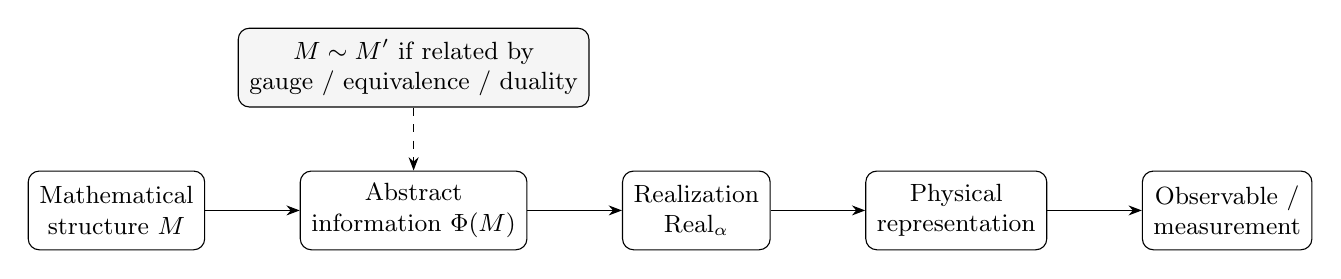
\begin{tikzpicture}[
  node distance=6mm and 12mm,
  box/.style={draw, rounded corners, align=center, minimum height=10mm,
              inner sep=4pt, font=\small},
  >={Stealth[]}]
\node[box] (M)  {Mathematical\\ structure $M$};
\node[box, right=of M] (Phi) {Abstract\\ information $\Phi(M)$};
\node[box, right=of Phi] (Re) {Realization\\ $\Real_\alpha$};
\node[box, right=of Re] (Pr) {Physical\\ representation};
\node[box, right=of Pr] (Ob) {Observable /\\ measurement};
\node[box, above=8mm of Phi, fill=gray!8] (Eq)
  {$M\sim M'$ if related by\\ gauge / equivalence / duality};
\draw[->] (M) -- (Phi);
\draw[->] (Phi) -- (Re);
\draw[->] (Re) -- (Pr);
\draw[->] (Pr) -- (Ob);
\draw[->, dashed] (Eq) -- (Phi);
\end{tikzpicture}
\caption{The spine: Part~\PI's realization pipeline, computing
$\Obs_\alpha(M)=\Obs(\Real_\alpha(\Phi(M)))$, with the gauge/equivalence datum
(\Cref{ax:equiv}) feeding the abstract-information step. Every module of the
library is a concrete instance of this diagram.}
\label{fig:spine}
\end{figure}

\subsection{The status calculus}
\label{sec:statuscalc}

The status labels are ordered $\Sstat\stle\Hstat\stle\Pstat$ (``standard is stronger
than heuristic is stronger than speculative'').  Part~\PI\ (\PI/T3) makes this a
\emph{calculus}: on $\{\Sstat,\Hstat,\Pstat\}$ put the commutative idempotent monoid
structure with unit $\Sstat$ and product $\max$ under $\stle$.  Then the composite of
representation entries $E_1,E_2$ (when $\tau_2\circ\tau_1$ is defined) has status
$\sigma_1\vee\sigma_2:=\max(\sigma_1,\sigma_2)$: \emph{status cannot improve under
composition; a chain of translations is only as reliable as its weakest link}.  This
observation, which is checkable and lends itself to mechanized propagation, governs
every composite we form in \Cref{sec:ladder,sec:closure}, and it is the reason the
Closure Theorem must carefully track the status of each ingredient.

% ==================================================================
\section{The modular composition ladder}
\label{sec:ladder}

We now traverse the ladder.  For each rung we state (i) the new structure introduced,
(ii) which spine axiom or definition of \Cref{sec:spine} it instantiates or
discharges, and (iii) --- the point of the whole exercise --- the single
\emph{emergent representational property} that appears only in the composite.  The
emergent properties are collected in \Cref{tab:ladder}.

\subsection{Rung \texorpdfstring{$\PI$}{I}: the possibility of disciplined translation}

Part~\PI\ introduces the primitives themselves: $\Dom,\Math_d,\Phys$, the
representation entry $(M,P,\tau,\sigma)$, the prestack/stack, the pipeline
\eqref{eq:pipeline}, and the status system.  There is as yet nothing to compose;
the emergent contribution of the base rung is \emph{the very possibility of a
disciplined mathematics$\leftrightarrow$physics translation}: syntax (the
mathematics), semantics (the physical role), and epistemic warrant (the status) are,
for the first time, tracked as \emph{data} rather than prose.  This is what makes the
later emergences \emph{sayable}.

\subsection{Rung \texorpdfstring{$\PI\to\PII$}{I to II}: coalgebraic anatomy}
\label{sec:rung2}

Part~\PII\ makes $\Real_\alpha$ concrete.  The abstract-information step becomes
$\Phi(X)=\Mot(X)$; the realization channels become the honest functors
$\Real_\alpha\in\{\text{Betti},\text{de Rham},\text{Hodge},\text{\'etale}\}$ with
$H_\alpha(X)\simeq\Real_\alpha(\Mot(X))$; and $\Obs$ becomes the period
$\per(\Pi)=\int_\Gamma\omega$ of a period datum $\Pi=(X,D,\omega,\Gamma)$.  The master
refinement is
\begin{equation}
\label{eq:ampl}
\Amp=\per(\Ampm),
\qquad
\Delta(\Ampm)=\textstyle\sum_i \Ampm_{i,1}\otimes\Ampm_{i,2},
\qquad
\delta:\Lcoalg\to\Lcoalg\wedge\Lcoalg,
\end{equation}
with $\Ampm$ a motivic amplitude object in a comodule over a Hopf algebra of motivic
periods.  Part~\PII's central proposition (\PII/T1) is that a monoidal realization
functor transports the coaction: $\Real_\alpha(\Delta(a))=(\Real_\alpha\otimes
\Real_\alpha)(\Delta(a))$, so the decomposition of $\Ampm$ descends to a decomposition
of the analytic/numerical amplitude.  This \emph{instantiates} \Cref{ax:dec}
(Decomposition) exactly.

\paragraph{Emergent property.}
Composing \PI\ with \PII\ endows observables with an internal \emph{coalgebraic
anatomy}: an amplitude is no longer an opaque number but a structured object that
\emph{decomposes} into primitive informational pieces (weight-graded polylogarithmic
generators, \PII/T2), and this anatomy is stable under any compatible realization
channel.  Numerical measurement and structural decomposition become two views of one
object.  Status: the transport is \Sstat/\Hstat\ (formal for comodules; physical only
when the amplitude admits a motivic lift), with the elliptic/non-Tate obstruction
(\PII/T4) a genuine \Sstat\ limitation theorem and the cosmic Galois functoriality
(\PII/T5) explicitly \Hstat/\Pstat.

\subsection{Rung \texorpdfstring{$\PII\to\PIII$}{II to III}: geometric variation}
\label{sec:rung3}

A period datum requires $X$ to be an \emph{actual} algebraic/analytic space, and a
family of amplitudes over kinematic space is a \emph{variation} of that data.
Part~\PIII\ supplies the stage: schemes and $\Spec R$, the on-shell observable
algebra $R/I$, moduli spaces and stacks, and --- crucially --- variations of Hodge
structure with the Gauss--Manin connection.  Part~\PIII/T1 upgrades \PII's per-object
pipeline to a \emph{family} pipeline: the assignment $s\mapsto
\Real_{\text{Hodge}}(\Mot(X_s))$ is a flat section of a variation of Hodge structure
over the base $S$, and the periods satisfy the Picard--Fuchs equation
$\nabla\,\Pi(s)=0$.  Positive geometries add a second, geometric decomposition
principle: the residue of a canonical form along a boundary is the canonical form of
the boundary geometry (\PIII/T3), conjecturally isomorphic to \PII's coaction tree.

\paragraph{Emergent property.}
The composite exhibits \emph{geometric variation of physical possibility}: motives and
periods are now understood as living over and varying across concrete moduli, so
``physical possibility'' acquires a geometric object --- the moduli space itself, its
singularities (thresholds), and its compactification (asymptotic states).  Amplitudes
become flat sections; analytic continuation becomes monodromy; a differential equation
(Picard--Fuchs) governs the whole family.  The decomposition axiom now has \emph{two}
independent geometric realizations (motivic coaction and positive-geometry residue),
whose conjectured coincidence (\PIII/T3, status \Hstat) is the programme's most
interesting open problem (\Cref{sec:open}).

\subsection{Rung \texorpdfstring{$\PIII\to\PIV$}{III to IV}: functorial conservation}
\label{sec:rung4}

Geometric spaces carry topological invariants stable under continuous deformation.
Part~\PIV\ supplies (co)homology, characteristic classes, bordism, and --- the
decisive step --- TQFT as a symmetric monoidal functor $Z:\Bord_n\to\Vect$.
Part~\PIV/T1 identifies $Z$ as a bona fide representation entry
$(\Bord_n,\Vect,Z,\Sstat)$ in the sense of \Cref{def:entry}, with $\Phi$ sending a
physical scenario to the underlying closed $(n{-}1)$-manifold (its boundary object) on
which the theory acts, $\Real_\alpha=Z$, and $\Obs$ the dimension/trace; the
symmetric monoidal (covariant) functoriality $Z(M_1\sqcup M_2)=Z(M_1)\otimes Z(M_2)$,
$Z(M_1\circ M_2)=Z(M_1)\circ Z(M_2)$ is precisely \Cref{ax:dec} for disjoint unions
and gluing.  The Atiyah--Singer index theorem $\mathrm{ind}(D)=\int_X\hat A(X)\wedge
\mathrm{ch}(E)$ (\PIV/T3) is an unimpeachably \Sstat\ instance of the master formula
$\text{observable}=\Real(\text{abstract structure})$.

\paragraph{Emergent property.}
The composite yields \emph{functorial conservation}: realization becomes a functor
over cobordisms, so ``the same physics'' is now transported \emph{coherently} along
histories, and topological invariants (charges, anomalies, phases) emerge as data that
\emph{no local deformation can change}.  This is also the first appearance of category
theory as the ambient grammar: TQFT is the historically first fully rigorous,
status-\Sstat\ instance of the pipeline as a functor, and the cobordism hypothesis
(\PIV/T2) --- extended TQFTs are classified by their value on a point --- announces the
extreme compositional rigidity that Part~\PV\ will abstract.

\subsection{Rung \texorpdfstring{$\PIV\to\PV$}{IV to V}: universal compositional grammar}
\label{sec:rung5}

Part~\PIV\ \emph{exhibited} one rigorous ``physics as a functor.''  Part~\PV\ supplies
the \emph{general theory} in which that instance and every other realization functor
lives: categories, functors, natural transformations, monoidal and dagger-compact
structure, and the homotopy-type-theoretic layer of identity types and univalence.
Two discharges occur here.  First, \PV/T2 (Curry--Howard--Lambek) gives a categorical
semantics for the whole pipeline as a single composite functor
$\mathsf{TypeTheory}\to\Phys$, simultaneously interpreting logic, code, and physical
representation.  Second, and centrally, \PV/T1 turns \Cref{ax:equiv} from a
\emph{postulate} into a \emph{theorem}: univalence $(A=B)\simeq(A\simeq B)$ forces any
internally definable realization to identify equivalent structures.  Dagger-compact
categories additionally give a self-contained categorical no-cloning theorem (\PV/T3),
which will \emph{force} Part~\PVI's encoding-based definition of high availability.

\paragraph{Emergent property.}
The composite makes the implicit functoriality of \PIV\ into an \emph{explicit
universal grammar of composition and identity}.  Equivalence of representations is now
\emph{provably} respected (univalence), not merely stipulated; the gap between
gauge-dependent and gauge-invariant quantities becomes the precise gap between
externally and internally definable realizations.  This is the rung at which the
library becomes self-describing: its own translations are objects of the theory it
studies.

\subsection{Rung \texorpdfstring{$\PV\to\PVI$}{V to VI}: gauge / fault-tolerant high availability}
\label{sec:rung6}

Part~\PVI\ is the capstone.  Using \PV's fibered categories and groupoid quotients it
\emph{defines rigorously} what Part~\PI\ merely posited: a stack is a fibered category
satisfying descent for a Grothendieck topology, and the quotient stack $[X/G]$ retains
isotropy, $\Aut_{[X/G]}(x)\simeq\Stab_G(x)$.  It then unifies two families of
``many descriptions, one content'' phenomena: gauge redundancy $[X/G]$ (the coarse
quotient $X/G$ forgets the stabilizers that carry anomaly and path-integral weight),
and quantum high-availability encodings $\iota:\Hlog\hookrightarrow\Hphys$ with the
subsystem decomposition
\begin{equation}
\label{eq:qha}
\Hphys\;\simeq\;(\Hlog\otimes\Hgauge)\;\oplus\;\Herr .
\end{equation}
For surface codes (\PVI/T3), logical operators are the nontrivial homology classes
$H_1(\Sigma;\ZZ_2)$ of the code surface --- a \emph{literal}, status-\Sstat\ reuse of
Part~\PIV's homology dictionary entry.  Renormalization reappears as the antipode of
the Connes--Kreimer Hopf algebra (\PVI/T4), reusing \PII's coalgebra on a different
combinatorial substrate.

\paragraph{Emergent property.}
The composite delivers \emph{high availability / fault tolerance}: gauge/quotient
constructions and quantum error-correcting codes are one representational phenomenon
--- many physical representatives realize one logical/observable content, robustly
against a controlled class of variations.  This is the property the entire ladder was
climbing toward, and its two faces (gauge redundancy, quantum encoding) are identified
by the isotropy correspondence at the heart of the Closure Theorem
(\Cref{sec:closure}).

\begin{table}[t]
\centering
\renewcommand{\arraystretch}{1.32}
\small
\begin{tabular}{@{}p{0.055\textwidth}p{0.29\textwidth}p{0.24\textwidth}p{0.30\textwidth}@{}}
\toprule
\textbf{Rung} & \textbf{New structure} & \textbf{Spine axiom
touched} & \textbf{Emergent property (composition adds)} \\
\midrule
\PI\ &
Entries $(M,P,\tau,\sigma)$; prestack/stack; pipeline; \Sstat/\Hstat/\Pstat\ &
all four posited &
Disciplined translation: syntax vs.\ semantics vs.\ status, tracked as data \\
\PII\ &
Motives; period data; $\Ampm$; coaction $\Delta$, cobracket $\delta$ &
\Cref{ax:dec} instantiated &
\emph{Coalgebraic anatomy}: observables decompose into primitive pieces \\
\PIII\ &
Schemes; moduli stacks; VHS; Gauss--Manin; positive geometries &
\Cref{ax:desc,ax:dec} refined &
\emph{Geometric variation}: possibilities live over and vary across moduli \\
\PIV\ &
(Co)homology; characteristic classes; bordism; TQFT $Z:\Bord_n\to\Vect$ &
\Cref{ax:real,ax:dec} realized &
\emph{Functorial conservation}: invariants stable under deformation; realization is a functor \\
\PV\ &
Functors; naturality; monoidal/dagger; identity types; univalence &
\Cref{ax:equiv} \emph{proved} &
\emph{Universal compositional grammar}: equivalence provably respected \\
\PVI\ &
Sheaves; stacks; $[X/G]$; QEC codes; Hopf renormalization &
\Cref{ax:desc,ax:equiv} \emph{discharged} &
\emph{High availability / fault tolerance}: many representatives, one content \\
\bottomrule
\end{tabular}
\caption{The modular composition ladder.  Each rung introduces one new structure,
touches one or more spine axioms of \Cref{sec:spine}, and contributes one emergent
representational property that exists only in the composite.}
\label{tab:ladder}
\end{table}

% ==================================================================
\section{A unified mathematical framework}
\label{sec:framework}

Having traversed the ladder informally, we now give the single mathematical object in
which all six faculties sit, and the master commuting diagram that ties them together.
We stress once more (\Cref{sec:intro}) that ``unified'' here means \emph{assembled from
modular parts by a canonical construction}, not \emph{fused into one primitive}.

\subsection{The total representation category}

\begin{definition}[Total representation category]
\label{def:total}
Let $\Repphys:\Dom^\op\to\Gpd$ be the representation prestack (\Cref{def:prestack}).
Its \emph{Grothendieck construction} $\int_\Dom\Repphys$ is the category whose objects
are pairs $(d,E)$ with $d\in\Dom$ and $E\in\Repphys(d)$ a representation entry over
$d$, and whose morphisms $(d,E)\to(d',E')$ are pairs $(u,\phi)$ with $u:d\to d'$ in
$\Dom$ and $\phi:E\to u^*E'$ an isomorphism in $\Repphys(d)$.  The projection
$\pi:\int_\Dom\Repphys\to\Dom$, $(d,E)\mapsto d$, is a fibered category (a
Grothendieck fibration in groupoids), and $\Repphys$ is recovered as its groupoid of
sections.
\end{definition}

The Grothendieck construction is the categorical device that turns the domain-indexed,
\emph{local} data of the library into a single \emph{global} category without
collapsing the domain index --- exactly the modular discipline of \Cref{sec:intro}
made precise.  The six modules populate the fibers:
$\Repphys(\text{motives})$, $\Repphys(\text{alg.\ geom.})$,
$\Repphys(\text{alg.\ top.})$, $\Repphys(\text{cat/HoTT})$,
$\Repphys(\text{sheaf/stack})$ are the fibers over the corresponding domains.

\subsection{The global realization functor}

Each module supplies, over its fiber, a factorization of the pipeline
\eqref{eq:pipeline} through named categories.  Writing $\Info_d,\Rep_d,\Meas_d$ for
the abstract-information, physical-representation and measurement categories of domain
$d$, the module's content is a triple of functors
\[
\Math_d\ \xrightarrow{\ \Phi_d\ }\ \Info_d\
\xrightarrow{\ \Real^{(d)}_\alpha\ }\ \Rep_d\
\xrightarrow{\ \Obs_d\ }\ \Meas_d,
\]
whose composite $\Obs_d\circ\Real^{(d)}_\alpha\circ\Phi_d$ is a functor
$\Math_d\to\Meas_d\subseteq\Phys$ whenever each factor is functorial (Part~\PI/T1).
The following are the six instances, each pinned to its status:

\begin{center}
\renewcommand{\arraystretch}{1.28}
\small
\begin{tabular}{@{}llll@{}}
\toprule
Module & $\Phi_d$ & $\Real^{(d)}_\alpha$ & $\Obs_d$ \\
\midrule
\PII\ & $X\mapsto\Mot(X)$ & Betti/de~Rham/Hodge/\'etale & period $\per(\Pi)=\int_\Gamma\omega$ \\
\PIII\ & family $X_s\mapsto$ VHS & Gauss--Manin flat transport & flat section / monodromy \\
\PIV\ & closed $(n{-}1)$-manifold & TQFT functor $Z:\Bord_n\to\Vect$ & dimension / trace / index \\
\PV\ & type $A:\mathcal U$ & internal construction & term extraction / global sections \\
\PVI\ & logical data $\Hlog$ & encoding $\iota:\Hlog\hookrightarrow\Hphys$ & syndrome / logical readout \\
\bottomrule
\end{tabular}
\end{center}

By the status calculus (\Cref{sec:statuscalc}), the status of a \emph{composite}
realization is the $\max$ over its three factors: a module's realization is
status-\Sstat\ only when all three functors are honestly constructed (as for TQFT), and
degrades to \Hstat\ or \Pstat\ as soon as any factor is merely interpretive or
speculative.

\subsection{The master commuting diagram}

\Cref{fig:master} assembles the six faculties.  The left column is the ladder: the
builds-on functors $J_{d,d+1}:\Math_d\to\Math_{d+1}$ realize each module as living
inside the next (motivic amplitude objects are objects of a derived category of motives
of a variety of \PIII; the moduli space of \PIII\ has the (co)homology of \PIV;
TQFT is an instance of \PV's functor grammar; \PV's fibered categories are the raw
material of \PVI's stacks).  Every module realizes into the single target $\Phys$
through its global realization functor $\Real_d$, and the triangles commute because
realization is compatible with the builds-on functors: realizing at a higher level and
then restricting agrees with realizing at the lower level.  The dashed arrow closes the
ladder: Part~\PVI's stackification proves that the top of the tower, Part~\PI's
representation stack, exists (\Cref{sec:closure}).

\begin{figure}[t]
\centering
\begin{tikzcd}[row sep=2.55em, column sep=7.5em]
\Math_{\mathrm{I}}
  \arrow[d, "J_{12}"']
  \arrow[r, "\Real_{\mathrm{I}}"]
  & \Phys \\
\Math_{\mathrm{II}}
  \arrow[d, "J_{23}"']
  \arrow[ur, "\Real_{\mathrm{II}}"']
  & \\
\Math_{\mathrm{III}}
  \arrow[d, "J_{34}"']
  \arrow[uur, "\Real_{\mathrm{III}}"' near end]
  & \\
\Math_{\mathrm{IV}}
  \arrow[d, "J_{45}"']
  \arrow[uuur, "\Real_{\mathrm{IV}}" near end]
  & \\
\Math_{\mathrm{V}}
  \arrow[d, "J_{56}"']
  \arrow[uuuur, "\Real_{\mathrm{V}}" near end]
  & \\
\Math_{\mathrm{VI}}
  \arrow[uuuuur, "\Real_{\mathrm{VI}}"' near end]
  \arrow[uuuuu, dashed, bend right=58,
         "\substack{\text{stackify}\\ \text{(closure, T2)}}"']
  &
\end{tikzcd}
\caption{The master commuting diagram of the library.  Vertical: the builds-on
functors $J_{d,d+1}$ (the ladder).  Diagonal: the global realization functors
$\Real_d:\Math_d\to\Phys$, forming a cocone over the single physical target
$\Phys$; each triangle
$\Real_{d+1}\circ J_{d,d+1}\Rightarrow\Real_d$ commutes up to coherent isomorphism
(realization is compatible with refinement).  Dashed: Part~\PVI's stackification
carries the final rung ($\Math_{\mathrm{VI}}$) back to Part~\PI, closing the ladder
(\Cref{thm:closure}).}
\label{fig:master}
\end{figure}

\subsection{The master formulas as one system}
\label{sec:masterformulas}

The programme has a small set of recurring formulas.  In the unified framework they are
one system, read off the total category and its fibers:
\begin{align}
\physrep{M} &:= \text{physical representation of }M
   && \text{(bracket; \Cref{def:entry})} \label{eq:mf1}\\
\Obs_\alpha(M) &= \Obs(\Real_\alpha(\Phi(M)))
   && \text{(pipeline; \Cref{ax:real})} \label{eq:mf2}\\
\text{observable} &= \Real(\text{abstract structure})
   && \text{(master slogan)} \label{eq:mf3}\\
\Amp &= \per(\Ampm)
   && \text{(motivic pre-numericality; \PII)} \label{eq:mf4}\\
\Delta(\Ampm) &= \textstyle\sum_i \Ampm_{i,1}\otimes\Ampm_{i,2}
   && \text{(coaction / full anatomy; \PII,\PVI)} \label{eq:mf5}\\
\delta &: \Lcoalg\to\Lcoalg\wedge\Lcoalg
   && \text{(cobracket / primitive split; \PII)} \label{eq:mf6}\\
\Aut_{[X/G]}(x) &\simeq \Stab_G(x)
   && \text{(isotropy retention; \PI,\PIII,\PV,\PVI)} \label{eq:mf7}\\
\Hphys &\simeq (\Hlog\otimes\Hgauge)\;\oplus\;\Herr
   && \text{(high-availability decomposition; \PVI)} \label{eq:mf8}
\end{align}
Formulas \eqref{eq:mf1}--\eqref{eq:mf3} are the spine; \eqref{eq:mf4}--\eqref{eq:mf6}
are its decomposition refinement; and \eqref{eq:mf7}--\eqref{eq:mf8} are the isotropy
and high-availability pair that the Closure Theorem identifies.  \Cref{tab:masterrec}
records how each module's central theorem is a special case of one of these formulas.

\begin{table}[t]
\centering
\renewcommand{\arraystretch}{1.3}
\small
\begin{tabular}{@{}llp{0.45\textwidth}@{}}
\toprule
Module theorem & Master formula & Sense of specialization \\
\midrule
\PI/T1 (pipeline is a functor) & \eqref{eq:mf2} & functoriality of $\Obs\circ\Real_\alpha\circ\Phi$ \\
\PII/T1 (coaction transport) & \eqref{eq:mf5} & $\Real_\alpha$ monoidal $\Rightarrow$ carries $\Delta$ \\
\PII/T2 (weight primitives) & \eqref{eq:mf6} & $\delta$ generates $\Lcoalg$ from weight-$1$ \\
\PIII/T1 (Gauss--Manin) & \eqref{eq:mf2} & pipeline fibered over moduli, flat section \\
\PIII/T3 (positive-geometry residue) & \eqref{eq:mf5} & residue tree $\cong$ coaction tree (conj., \Hstat) \\
\PIV/T1 (TQFT is an entry) & \eqref{eq:mf2},\eqref{eq:mf3} & $Z=\Real_\alpha$, $\Obs=$ trace \\
\PIV/T3 (index theorem) & \eqref{eq:mf3} & $\mathrm{ind}(D)=\Real_{\text{top}}(\text{char.\ classes})$ \\
\PV/T1 (univalence) & \eqref{eq:mf7} & equivalence $=$ identity for internal $\Real$ \\
\PVI/T1 (stacks retain isotropy) & \eqref{eq:mf7} & $\Aut_{[X/G]}(x)\simeq\Stab_G(x)$ \\
\PVI/T3 (surface code) & \eqref{eq:mf8} & $\Hlog\cong H_1(\Sigma;\ZZ_2)$ \\
\PVI/T4 (Connes--Kreimer antipode) & \eqref{eq:mf5} & $\Delta$ on graphs, antipode $=$ counterterm \\
\bottomrule
\end{tabular}
\caption{Each module's central theorem as a special case of a master formula
\eqref{eq:mf1}--\eqref{eq:mf8}.  This is the quantitative content of ``the whole
machinery is recovered module by module.''}
\label{tab:masterrec}
\end{table}

% ==================================================================
\section{Cross-cutting themes}
\label{sec:crosscut}

Certain items recur across two or more modules; these are the load-bearing joints of
the synthesis.  We treat five.

\subsection{One realization formula, six instances}

The pipeline \eqref{eq:mf2} is the single backbone formula, instantiated concretely by
every module (the $\Phi_d,\Real^{(d)}_\alpha,\Obs_d$ table of \Cref{sec:framework}).
The instances are not analogies: in \PIV\ the realization functor is literally a TQFT;
in \PII\ it is literally a period; in \PVI\ it is literally a quantum encoding.  What
varies is only the epistemic status of the composite, governed by the status calculus.
This is why the library can be simultaneously ambitious (one formula for all of
physical representation) and honest (each instance is graded).

\subsection{One Hopf/coalgebra of decomposition}
\label{sec:onehopf}

\Cref{ax:dec} (Decomposition) has a strikingly uniform incarnation.  Every module
supplies a decomposition operation, and all are instances of a single algebraic
pattern: a \emph{graded connected Hopf/coalgebra structure with a primitive-antisymmetric
part}.

\begin{principle}[Universal decomposition]
\label{prin:dec}
The decomposition operations of the library --- the motivic coaction $\Delta$ and
Goncharov cobracket $\delta$ (\PII); the positive-geometry residue (\PIII); the
boundary operator $\partial$ and the long exact/spectral sequences (\PIV); and the
Connes--Kreimer coproduct with antipode $S$ (\PVI) --- are all realizations of one
graded, connected coalgebra-with-primitives, differing only in the combinatorial data
they act on (polylogarithm symbols, boundary strata, chains, rooted trees).
\end{principle}

Two facts make \Cref{prin:dec} more than a slogan.  First, \PII\ and \PVI\ literally
share references: Connes--Kreimer \cite{ConnesKreimer1999} and Goncharov
\cite{Goncharov2005} appear in both reference pools, and both are graded connected Hopf
algebras with antipode --- one on rooted trees (subdivergences), one on polylogarithm
symbols (transcendentality).  Second, the antipode formula of \PVI/T4,
$S(\Gamma)=-\Gamma-\sum S(\Gamma')\,(\Gamma/\Gamma')$, is the exact algebraic dual of
the recursive residue of \PIII/T3 and of the iterated coaction of \PII: subtraction of
subdivergences, restriction to boundary strata, and extraction of primitive pieces are
one operation in three costumes.  The conjectural equality of the motivic coaction tree
and the positive-geometry residue tree (\PIII/T3) is the sharpest open instance of this
principle (\Cref{sec:open}), and we flag it status \Hstat.

\subsection{A functoriality gradient of increasing concreteness}

Functoriality of realization threads the ladder at three increasing levels of concreteness:
Part~\PI\ \emph{posits} it (\Cref{ax:real}, $\Real_\alpha$ implicitly functorial);
Part~\PIV\ \emph{exhibits} the first fully rigorous instance (TQFT $Z:\Bord_n\to\Vect$,
\PIV/T1, status \Sstat); Part~\PV\ supplies the \emph{general theory} (functors,
natural transformations, the whole grammar, \PV/T2).  The cobordism hypothesis
(\PIV/T2) is the historical hinge: it is a topological, status-\Sstat\ theorem whose
proof \emph{requires} the higher-categorical duality data that Part~\PV\ formalizes, so
it simultaneously closes Part~\PIV\ and motivates Part~\PV.

\subsection{The isotropy theorem, four proofs}
\label{sec:isotropy}

The single most recurrent theorem of the library is the retention of automorphism
(stabilizer) data by the stack quotient, \eqref{eq:mf7}.  It appears \emph{four} times,
at strictly increasing rigor:

\begin{enumerate}[leftmargin=2.2em]
\item \textbf{Part~\PI\ (informal).}  The representation stack (\Cref{def:stack}) glues
entries ``not by equality but by equivalence,'' with automorphisms modeling gauge and
duality --- a posited property.
\item \textbf{Part~\PIII\ (algebro-geometric, \PIII/T2).}  If $x$ has stabilizer
$\Stab_G(x)\neq 1$, the coarse map $[X/G]\to X/G$ is not an isomorphism near $x$; the
local structure of $[X/G]$ at $x$ is $[\Spec\mathcal O_{X,x}/\Stab_G(x)]$, recording
exactly the data lost by $X/G$.
\item \textbf{Part~\PV\ (type-theoretic, \PV/T4).}  The set quotient $X/G$ (a
$0$-type) forgets the path (automorphism) data that the groupoid quotient $X/\!\!/G$
(a $1$-type when stabilizers are discrete) retains as nontrivial loops; passing
$X\rightsquigarrow[X/G]$ is passing from a $0$-type to a $1$-type in the truncation
hierarchy.
\item \textbf{Part~\PVI\ (descent-theoretic, \PVI/T1).}  The local structure of
$[X/G]$ at $x$ is the classifying stack $[\ast/\Stab_G(x)]$, whose every point has
automorphism group $\Stab_G(x)$; the coarse-space functor collapses $\Aut$ to the
trivial group, so any observable counting automorphisms (orbifold Euler characteristic,
$1/|\Stab|$ path-integral weight) is computable from $[X/G]$ but not from $X/G$.
\end{enumerate}

These are not four theorems but one theorem with four proofs, and the synthesis
presents them as such: this is the axis of the Closure Theorem (\Cref{sec:closure}).

\subsection{Homology reused literally}

Part~\PIV's abstract dictionary entry ``homology $H_n(X)$ $\leftrightarrow$ conserved
extended structures'' becomes, in Part~\PVI, a concrete quantum-information mechanism:
for a surface code on a genus-$g$ surface $\Sigma$, the logical operators are the
generators of $H_1(\Sigma;\ZZ_2)$ and the code space is $(\CC^2)^{\otimes 2g}$
(\PVI/T3).  Contractible error strings are boundaries and act trivially --- exactly the
Part~\PIV\ entry ``boundary $c=\partial b$ $\leftrightarrow$ pure gauge / physically
null sector.''  This is direct literal reuse, not analogy, and it is the strongest
(status-\Sstat) bridge in the entire library between algebraic topology, gauge/stacks,
and quantum information.

% ==================================================================
\section{The Closure Theorem}
\label{sec:closure}

We now state and assemble the headline result.  It has three faces: a
descent-theoretic statement that the representation stack \emph{exists}, an isotropy
statement that unifies its four proofs, and a physical statement that identifies gauge
redundancy with quantum high availability.

\subsection{Statement}

\begin{theorem}[Closure Theorem]
\label{thm:closure}
Let $(\Dom,J)$ be the site of mathematical domains and
$\Repphys:\Dom^\op\to\Gpd$ the representation prestack of Part~\PI\
(\Cref{def:prestack}), whose local data over the domains
$\{\text{motives},\text{alg.\ geom.},\text{alg.\ top.},\text{cat/HoTT},
\text{sheaf/stack}\}$ are supplied concretely by Parts~\PII--\PVI\ (periods and
coactions; VHS and Gauss--Manin; (co)homology and TQFT functors; identity data and
univalence; encodings and stabilizers).  Then:
\begin{enumerate}
\item \textup{(Existence, status \Sstat/\Hstat.)}  There is a stack
$\Repphys^{J}$ on $(\Dom,J)$ and a universal morphism $\eta:\Repphys\to\Repphys^{J}$
such that for every stack $\mathcal G$, precomposition
\[
\eta^*:\ \iHom_{\mathrm{Stack}}(\Repphys^{J},\mathcal G)\ \xrightarrow{\ \simeq\ }\
\iHom_{\mathrm{CFG}}(\Repphys,\mathcal G)
\]
is an equivalence of groupoids
\textup{(Part~\PVI/T2)}.  Consequently Part~\PI's ``representation stack''
\textup{(\Cref{def:stack})} exists and equals $\Repphys^{J}$: when the local
realization data of Parts~\PII--\PV\ agree on overlaps they assemble into a global
object of $\Repphys^{J}$, exactly satisfying the informal gluing of
\Cref{def:stack,ax:desc}.
\item \textup{(Closure under the six operations, status \Sstat.)}  $\Repphys^{J}$ is
closed under the five library operations of \Cref{def:library} --- restriction,
transport, composition, decomposition, realization --- interpreted through the six
faculties: restriction is $J$-refinement; transport is univalence-respecting
equivalence \textup{(\PV/T1)}; composition is functor composition with status
$\max$-propagation \textup{(\PI/T3)}; decomposition is the universal
coalgebra/coaction of \Cref{prin:dec} \textup{(\PII,\PIII,\PIV,\PVI)}; and
realization is the global functor of \Cref{sec:framework} \textup{(\PIV)}.
\item \textup{(Isotropy keystone, status \Sstat.)}  For every gauge datum
$(X,G)$ occurring in a fiber and every $x\in X$,
\[
\Aut_{\,\Repphys^{J}}(x)\ \simeq\ \Aut_{[X/G]}(x)\ \simeq\ \Stab_G(x),
\]
a single isomorphism established four independent ways \textup{(\PI,\PIII/T2,
\PV/T4,\PVI/T1; \Cref{sec:isotropy})}.  Its physical face is the equivalence of
\emph{gauge redundancy} and \emph{quantum high availability}: the encoding
$\iota:\Hlog\hookrightarrow\Hphys$ with $\Hphys\simeq(\Hlog\otimes\Hgauge)\oplus\Herr$
\eqref{eq:mf8} presents the same ``many representatives, one logical content''
structure as the quotient stack, with $\Hgauge$ the isotropy/gauge directions and
$\Herr$ the syndrome sectors \textup{(\PVI/T3)}.
\end{enumerate}
\end{theorem}

\begin{proof}[Assembly]
Part~(1) is Part~\PVI/T2 verbatim: one adapts the plus construction from set-valued to
groupoid-valued coefficients, setting
$\Repphys^{+}(U)=\varinjlim_{\{U_i\to U\}\in J(U)}
\mathrm{Desc}(\{U_i\to U\},\Repphys)$ over the filtered category of covers of $U$
(any two covers admit a common refinement by pairwise pullbacks), and
$\Repphys^{J}:=\Repphys^{++}$; then $\Repphys^{+}$ is a prestack for any fibered
category in groupoids and a stack when $\Repphys$ is already a prestack, and the
universal property
follows because descent in the target stack $\mathcal G$ makes every descent datum
effective, yielding the essentially unique factorization through $\eta$.  This is the
general stackification theorem for fibered categories over a site
\cite{Giraud1971,Vistoli2004}, specialized to $\Repphys$; the mathematics is
status-\Sstat, and only the modeling claim that the Parts~\PII--\PV\ realization data
\emph{is} a $J$-descent datum is status-\Hstat\ (\Cref{sec:limitations}).

Part~(2) reads off the five closure operations from the six modules.  Closure under
restriction and realization is definitional for a stack.  Closure under transport is
Part~\PV/T1: an internally definable realization cannot distinguish equivalent
$A\simeq B$, since univalence gives a path $A=B$ and path induction (the $J$-rule)
transports every construction; hence equivalence-related entries have equal image.
Closure under composition, with status tracked, is Part~\PI/T3: the composite of two
entries has status $\max(\sigma_1,\sigma_2)$ under $\Sstat\stle\Hstat\stle\Pstat$, so
$\Repphys^{J}$ is closed as a status-graded category (a lax monoidal functor to
$(\{\Sstat,\Hstat,\Pstat\},\max)$).  Closure under decomposition is
\Cref{prin:dec}: each fiber carries its coalgebra of decomposition (motivic coaction,
residue, boundary, antipode), and these are compatible with realization by the
monoidality of \PII/T1 and the symmetric-monoidal gluing of the TQFT of \PIV/T1.

Part~(3) is the isotropy correspondence of \Cref{sec:isotropy}, whose four proofs
agree, together with its physical face.  The stack $\Repphys^{J}$ retains automorphisms
by construction (it is groupoid-valued), and for a gauge datum $(X,G)$ the fiber
automorphism group at $x$ is $\Stab_G(x)$ by Part~\PVI/T1.  The identification with
quantum high availability is Part~\PVI's Remark on the sheaf/stack/code analogy made
literal by Part~\PVI/T3: a stabilizer code stores logical data across physical degrees
of freedom together with transformations (stabilizers, gauge automorphisms) that do not
change the logical content, so the code space is the ``logical fiber'' of an encoding
stack, with $\Stab_G(x)\leftrightarrow$ stabilizer group $\leftrightarrow \Hgauge$ and
error sectors $\leftrightarrow\Herr$.  For surface codes this identification is exact
and status-\Sstat\ (logical operators $=H_1(\Sigma;\ZZ_2)$); the general slogan
``gauge redundancy is to physics what fault-tolerant encoding is to quantum
information'' is status-\Hstat\ (\Cref{sec:limitations}, \Cref{sec:open}).
\end{proof}

\begin{corollary}[The ladder closes]
\label{cor:closure}
The six modules are not merely an expository decomposition.  \Cref{thm:closure}(1)
shows that Part~\PI's \emph{opening} definition (the representation stack) is a
\emph{theorem} provable from Part~\PVI's descent machinery applied to the concrete data
of Parts~\PII--\PV.  The ladder $\PI\to\cdots\to\PVI$ therefore closes back onto
Part~\PI: what was posited at the base is discharged at the capstone.
\end{corollary}

\subsection{Why the keystone is forced, not chosen}

Part~\PV/T3 (categorical no-cloning) explains why the quantum face of the keystone must
be an \emph{encoding}, not a \emph{copy}.  In a dagger-compact category with biproducts
there is no natural diagonal $\Delta:A\to A\otimes A$ compatible with the
dagger-compact structure unless $A$ is classical (a special commutative
dagger-Frobenius algebra).  Hence classical high availability by \emph{replication} has
no quantum analogue; the only route to ``many physical representatives, one logical
content'' in the quantum setting is a genuine embedding
$\iota:\Hlog\hookrightarrow\Hphys$ into a larger, redundant system --- which is exactly
the gauge/stack structure of \eqref{eq:mf7}.  Part~\PV\ thus supplies the categorical
\emph{reason} that Part~\PVI's encoding-based definition is the correct one, and the
isotropy keystone is forced.

\begin{figure}[t]
\centering
\resizebox{\textwidth}{!}{%
\begin{tikzcd}[ampersand replacement=\&, row sep=large, column sep=1.6em]
\& \boxed{\text{Part \PI: } \Repphys \text{ posited stack-like}}
  \arrow[d, "\text{deferred}"] \& \\
\& \boxed{\text{Parts \PII--\PV: local realization data}}
  \arrow[d, "\text{descent datum}"] \& \\
\boxed{\text{gauge redundancy } [X/G]}
  \arrow[r, "\simeq"', "\Stab_G(x)"]
\& \boxed{\text{Part \PVI: stackify } \Repphys^{J}}
  \arrow[r, "\simeq"', "\Hgauge"]
  \arrow[uu, dashed, bend left=55, "\text{closes}"]
\& \boxed{\text{quantum HA } \iota:\Hlog\hookrightarrow\Hphys}
\end{tikzcd}%
}
\caption{The closure loop and its keystone.  Part~\PI\ posits and defers; Parts~\PII--\PV\
supply the local data as a descent datum; Part~\PVI\ stackifies to produce
$\Repphys^{J}$, which \emph{is} Part~\PI's stack (dashed ``closes'' arrow).  The
isotropy group $\Stab_G(x)$ identifies gauge redundancy (left) with quantum high
availability (right): $\Stab_G(x)\simeq\Hgauge$.}
\label{fig:closureloop}
\end{figure}

% ==================================================================
\section{Emergence, recomposed}
\label{sec:emergence}

We can now state precisely what ``emergence from composition'' means in this
programme, and check that the whole spine is recovered.

\begin{principle}[Emergence is compositional, not fundamental]
\label{prin:emerge}
Each emergent property of \Cref{tab:ladder} --- coalgebraic anatomy, geometric
variation, functorial conservation, universal grammar, high availability --- is a
property of a \emph{composite} of modules that is possessed by \emph{no single module}
in isolation.  Coalgebraic anatomy needs both the pipeline (\PI) and the coaction
(\PII); geometric variation needs both the coaction (\PII) and the moduli (\PIII);
functorial conservation needs both the moduli (\PIII) and the topological invariants
(\PIV); and so on.  The properties are therefore genuinely emergent in the technical
sense of arising at, and only at, a level of the composition hierarchy.
\end{principle}

The recomposition is complete in the following sense.  \Cref{tab:masterrec} exhibits
every module's central theorem as a special case of a master formula; \Cref{thm:closure}
shows the whole prestack of Part~\PI\ is recovered as the stackification of the concrete
data of Parts~\PII--\PVI; and \Cref{cor:closure} shows the recovery is \emph{exact}, in
that Part~\PI's own definition is satisfied.  Thus the informally posited Level-\PI\
structure is not merely \emph{illustrated} by the six modules --- it is
\emph{constructed} by them.  This is the precise content of the claim that the library
is a genuine hierarchical composition rather than a taxonomy.

% ==================================================================
\section{A quantitative status-label census}
\label{sec:status}

The status system is the library's epistemic-honesty device; here we make it
quantitative.  \Cref{tab:census} tabulates the status distribution of the principal
math$\to$physics dictionary table of each module (the shared cross-cutting operations
and domains-as-faculties tables of Part~\PI\ are excluded to avoid double counting; the
Part~\PVI\ quantum-information cross-dictionary is excluded because its entries carry
interpretive rather than \Sstat/\Hstat/\Pstat\ labels).  Composite labels are counted
in their own columns.

\begin{table}[t]
\centering
\renewcommand{\arraystretch}{1.25}
\begin{tabular}{@{}lrrrrr@{}}
\toprule
Module (principal dictionary) & \Sstat & \Sstat/\Hstat & \Hstat & \Hstat/\Pstat & Total \\
\midrule
\PI\ \ (core translation)        & 9  & 5  & 2  & 0 & 16 \\
\PII\ \ (motivic / amplitude)    & 20 & 9  & 2  & 1 & 32 \\
\PIII\ (algebraic geometry)      & 35 & 13 & 4  & 0 & 52 \\
\PIV\ (algebraic topology)       & 46 & 4  & 3  & 0 & 53 \\
\PV\ \ (category theory / HoTT)  & 26 & 31 & 18 & 0 & 75 \\
\PVI\ (Lie/Hopf/sheaf/stack)     & 26 & 12 & 2  & 0 & 40 \\
\midrule
\textbf{Total}                   & \textbf{162} & \textbf{74} & \textbf{31} & \textbf{1} & \textbf{268} \\
\bottomrule
\end{tabular}
\caption{Status-label census of the six principal dictionaries.  Of $268$ entries,
$162$ ($60.4\%$) are standard \Sstat, $74$ ($27.6\%$) are \Sstat/\Hstat\ (standard as
mathematics, heuristic in physical reading), $31$ ($11.6\%$) are heuristic \Hstat, and a
single entry (\PII's cosmic Galois group) is \Hstat/\Pstat.  No entry is purely
\Pstat: the library's speculative content lives in its \emph{theorems and conjecture},
not its dictionary.}
\label{tab:census}
\end{table}

Two patterns are worth reading off \Cref{tab:census}.  Part~\PIV\ (algebraic topology)
is the most \emph{standard} module ($87\%$ \Sstat): TQFT, index theory, and
characteristic classes are established mathematical physics.  Part~\PV\ (category
theory / HoTT) is the most \emph{interpretive} ($65\%$ \Sstat/\Hstat\ or \Hstat): its
mathematics is standard but its physical readings (a type as a space of states, a
functor as a physical theory) are heuristic by construction.  This is exactly as it
should be: the abstract compositional grammar is where physical interpretation is most
optional.

\paragraph{Status of the candidate theorems.}
The library's roughly thirty candidate theorems partition by status as follows.
\emph{Standard} (\Sstat): \PI/T1--T2, \PII/T1--T3, \PIII/T1--T2,T4, all of
\PIV/T1--T4, all of \PV/T1--T4, \PVI/T1--T4 --- these are either established results
reframed (Atiyah--Singer, Lurie's cobordism hypothesis, Giraud/Vistoli stackification,
Connes--Kreimer, univalence) or immediate consequences.  \emph{Original heuristic}
(\Hstat): \PI/T3 (the status calculus, original to the programme), \PIII/T3 (the
positive-geometry/coaction isomorphism, conjectural), and the general slogan ``gauge
redundancy $\cong$ fault-tolerant encoding'' beyond surface codes.  \emph{Speculative}
(\Pstat\ or \Hstat/\Pstat): \PII/T5 (functoriality of the cosmic Galois group action)
and the overarching Conjecture of \Cref{sec:open}.  The Closure Theorem
(\Cref{thm:closure}) is \Sstat\ in its mathematics and \Hstat\ in the modeling claim
that identifies the physical realization data with a descent datum.

% ==================================================================
\section{Limitations}
\label{sec:limitations}

The programme states five limitations, which we reproduce verbatim and then discuss
module by module.

\begin{enumerate}[leftmargin=2.2em, label=\textbf{L\arabic*.}]
\item Not every mathematical analogy is a physical theory --- status labels are part of
the formalism, not decoration.
\item Motives are NOT literally ``the functions of'' an object in standard mathematics;
that reading is this project's proposed semantic layer (status \Hstat), to be clearly
flagged in every module that uses it.
\item A single universal functor from all of mathematics to all of physics is unlikely
to be well-defined --- the representation-stack approach is deliberately
local/domain-indexed.  Modules should not overclaim a single functor
$\Math\to\Phys$.
\item Not every physical observable is known to be a period; some amplitudes require
elliptic, modular, non-Tate, or more general analytic structures.
\item Gauge redundancy $\neq$ physical symmetry: gauge symmetry identifies different
descriptions of the same physical content; physical symmetry maps one physical state to
a genuinely different one.
\end{enumerate}

\paragraph{Discussion.}
\textbf{L1} is honored globally by the status census (\Cref{sec:status}): the labels are
carried into every table and into the status calculus (\Cref{sec:statuscalc}), which
propagates them through composition.  \textbf{L2} constrains Part~\PII: the
functional-essence reading $\mathrm{FE}(X)=\Mot(X)$ is flagged \Hstat\ wherever it
appears, and the elliptic/non-Tate obstruction (\PII/T4) is a genuine \Sstat\ limitation
theorem, not a caveat.  \textbf{L3} is the reason the synthesis is \emph{modular}: the
unified framework of \Cref{sec:framework} is a Grothendieck construction over a
\emph{domain-indexed} prestack, precisely so as \emph{not} to assert a single global
functor; the closure of \Cref{thm:closure} is closure of a \emph{stack}, which lives
over the site $\Dom$ and never collapses the domain index.  \textbf{L4} bounds the
amplitude claims of Parts~\PII--\PIII: the master formula $\Amp=\per(\Ampm)$ is asserted
only for amplitudes admitting motivic lifts, and \PII/T4 delimits exactly where this
fails.  \textbf{L5} bounds the keystone of Part~\PVI\ and \Cref{thm:closure}(3): the
identification is of gauge \emph{redundancy} (descriptive freedom) with high
availability, \emph{not} of physical symmetry with high availability; the isotropy group
$\Stab_G(x)$ is a redundancy stabilizer, and physical symmetries --- which move between
genuinely distinct physical states --- are explicitly outside the scope of the keystone.

% ==================================================================
\section{Open problems and the research programme}
\label{sec:open}

The synthesis answers the source's own conjecture by listing the testable subprograms it
calls for.  We state the conjecture and the open problems.

\begin{conjecture}[Motivic--categorical information ontology, status \Pstat]
\label{conj:onto}
A sufficiently broad class of physical theories admits a representation-stack
description in which states, processes, observables, amplitudes, gauge redundancies,
and measurement values arise as realizations of structured categorical, homotopical,
geometric, and motivic information.
\end{conjecture}

The following are the concrete, citable open problems that would test
\Cref{conj:onto}, one per module.

\begin{itemize}[leftmargin=2.2em]
\item[\PI.] A fully rigorous stackification of the \emph{specific} groupoid
$\Repphys$ (as opposed to the general theorem of \PVI/T2) is original work; connections
to formalizations of ``prestacks of physical theories'' / ``stacks of QFTs'' (e.g.\
factorization homology, or Schreiber's cohesive-topos programme \cite{Schreiber2013})
remain to be made precise.
\item[\PII.] The precise definition of the cosmic Galois group for a general QFT (beyond
$\varphi^4$) remains conjectural; \PII/T5 is \Hstat/\Pstat\ pending post-2016 results in
the Panzer--Schnetz \cite{PanzerSchnetz2016} / Brown \cite{Brown2015Cosmic} line.
\item[\PIII.] The conjectural isomorphism between positive-geometry residue trees and
motivic coaction trees (\PIII/T3) is, to our knowledge, unproven in general; a ``Hopf
algebra of the amplituhedron'' would settle the sharpest instance of \Cref{prin:dec}.
\item[\PIV.] Identifying a \emph{given} SPT phase's bordism invariant (\PIV/T5) is
model-dependent; each lattice-model claim needs its own citation beyond the general
Freed--Hopkins classification \cite{FreedHopkins2016}.
\item[\PV.] Concrete cohesive-HoTT formalizations of specific gauge theories
(Yang--Mills, Chern--Simons) beyond Schreiber's general framework are largely
programmatic.
\item[\PVI.] The general claim ``gauge redundancy is to physics what fault-tolerant
encoding is to quantum information,'' beyond surface codes, is \Hstat; the holographic
quantum-error-correction / entanglement-wedge-reconstruction literature is the natural,
more rigorous body of work to strengthen it, and is the single largest opportunity for
a genuinely novel contribution.
\end{itemize}

% ==================================================================
\section{Conclusion}
\label{sec:conclusion}

We have recomposed the six modular parts of the library into one coherent account,
without collapsing them into a monolith.  The representation stack and realization
pipeline of Part~\PI\ are the spine; Parts~\PII--\PVI\ instantiate and progressively
discharge it; and at each rung of the composition ladder a single emergent property ---
coalgebraic anatomy, geometric variation, functorial conservation, universal grammar,
high availability --- arises from the composition and from nowhere else.  The Closure
Theorem (\Cref{thm:closure}) shows the ladder is genuinely circular: Part~\PI's
opening definition is a theorem of Part~\PVI, provable by descent-theoretic
stackification of the concrete data of the intervening modules, with the isotropy
correspondence $\Aut_{[X/G]}(x)\simeq\Stab_G(x)$ --- one theorem, four proofs --- as its
axis and \emph{gauge redundancy $\cong$ quantum high availability} as its keystone.

The programme's four compressed theses survive the synthesis intact, and we adopt them
as its closing summary:
\begin{quote}
\emph{mathematics is the syntax of physical representation;\\
motives are functional semantics;\\
periods are numerical measurements;\\
coalgebras are decomposition laws.}
\end{quote}
To these the ladder adds a fifth, which is the content of the capstone:
\emph{stacks are the grammar of redundancy, and redundancy, made robust, is high
availability.}

\section*{Acknowledgments}
This synthesis draws entirely on the six preceding parts of \emph{A \MtoP{}
Representation Library} and the shared knowledge base assembled for the series.  We
thank the YonedaAI Research Collective.

% ==================================================================
\appendix

\section{Unified operations dictionary}
\label{app:ops}

The following cross-cutting table (Part~\PI, Appendix~G) records the decomposition and
composition operations that recur across all modules, with the physical interpretation
each carries.  It is the concrete substance of \Cref{prin:dec}.

\begin{longtable}{@{}p{0.30\textwidth}p{0.62\textwidth}@{}}
\toprule
Operation & Physical interpretation (module) \\
\midrule
\endfirsthead
\toprule
Operation & Physical interpretation (module) \\
\midrule
\endhead
\bottomrule
\endfoot
Boundary $\partial$ & edge / flux / factorization (\PIV) \\
Differential $d$ & infinitesimal change (\PIII,\PIV) \\
Coboundary $d^{*}$ & gauge / exact shift (\PIV,\PVI) \\
Cobracket $\delta$ & primitive antisymmetric split (\PII) \\
Coproduct $\Delta$ & full split / coaction (\PII,\PVI) \\
Residue & pole / singular channel (\PII,\PIII) \\
Monodromy & analytic continuation (\PIII) \\
Filtration & scale hierarchy (\PII,\PVI) \\
Grading & charge / degree / loop / weight (\PII,\PIV,\PVI) \\
Spectral sequence & multi-scale obstruction (\PIV) \\
Localization & effective physics at a scale (\PIII) \\
Completion & perturbation expansion (\PIII) \\
Blowup & regularize divergence (\PIII) \\
Quotient & gauge reduction (\PIII,\PVI) \\
Pullback & constraint matching (\PV) \\
Pushout & couple systems (\PV) \\
Trace & partition function / loop amplitude (\PIV,\PV) \\
Dual & measurement / conjugate (\PV) \\
Tensor product $\otimes$ & parallel composition (\PIV,\PV) \\
Direct sum $\oplus$ & superselection (\PVI) \\
$\Hom$ & space of processes (\PV) \\
$\mathrm{Ext}$ & bound state / anomaly / deformation (\PIII,\PIV) \\
Antipode $S$ & counterterm / renormalization inverse (\PVI) \\
\end{longtable}

\section{Census methodology}
\label{app:census}

The counts of \Cref{tab:census} are obtained by tallying the status label of each row
of each module's \emph{principal} math$\to$physics dictionary (Part~\PI\ Appendix~A;
Part~\PII\ Appendix~B; Part~\PIII\ Appendix~C; Part~\PIV\ Appendix~D; Part~\PV\
Appendix~E, category-theory and HoTT tables merged; Part~\PVI\ Appendix~F,
Lie/Hopf/sheaf/stack table).  Composite labels are recorded in their own columns; a row
labeled \Sstat/\Hstat\ is counted once in the \Sstat/\Hstat\ column, not split.  The
Part~\PI\ cross-cutting operations table (Appendix~G, reproduced in \Cref{app:ops}) and
domains-as-faculties table (Appendix~H) are excluded to avoid double counting across
modules, and the Part~\PVI\ quantum-information cross-dictionary is excluded because its
entries carry interpretive rather than \Sstat/\Hstat/\Pstat\ labels.  These conventions
are deterministic and reproducible; the totals are $\Sstat=162$, $\Sstat/\Hstat=74$,
$\Hstat=31$, $\Hstat/\Pstat=1$, summing to $268$.

% ==================================================================
\begin{thebibliography}{99}

\bibitem{primary} M.~Long and the YonedaAI Collaboration, \emph{A \MtoP{}
Representation Library}, Parts~I--VI (this series), YonedaAI Research Collective, 2026.

\bibitem{Atiyah1988} M.~F. Atiyah, \emph{Topological quantum field theories},
Publ.\ Math.\ IH\'ES \textbf{68} (1988), 175--186.

\bibitem{Lurie2009} J.~Lurie, \emph{On the classification of topological field
theories}, in \emph{Current Developments in Mathematics 2008}, 129--280;
arXiv:0905.0465 (2009).

\bibitem{LurieHTT2009} J.~Lurie, \emph{Higher Topos Theory}, Annals of Mathematics
Studies \textbf{170}, Princeton University Press, 2009.

\bibitem{BaezStay2009} J.~C. Baez and M.~Stay, \emph{Physics, topology, logic and
computation: a Rosetta stone}, Lecture Notes in Physics \textbf{813} (2010), 95--172;
arXiv:0903.0340.

\bibitem{MacLane1998} S.~Mac Lane, \emph{Categories for the Working Mathematician},
2nd ed., Graduate Texts in Mathematics \textbf{5}, Springer, 1998.

\bibitem{AbramskyCoecke2004} S.~Abramsky and B.~Coecke, \emph{A categorical semantics
of quantum protocols}, Proc.\ 19th IEEE LiCS (2004); arXiv:quant-ph/0402130.

\bibitem{HoTT2013} The Univalent Foundations Program, \emph{Homotopy Type Theory:
Univalent Foundations of Mathematics}, Institute for Advanced Study, 2013.

\bibitem{RiehlVerity2022} E.~Riehl and D.~Verity, \emph{Elements of $\infty$-Category
Theory}, Cambridge Studies in Advanced Mathematics, Cambridge University Press, 2022.

\bibitem{LambekScott1986} J.~Lambek and P.~J. Scott, \emph{Introduction to Higher
Order Categorical Logic}, Cambridge Studies in Advanced Mathematics \textbf{7},
Cambridge University Press, 1986.

\bibitem{Schreiber2013} U.~Schreiber, \emph{Differential cohomology in a cohesive
$\infty$-topos}, arXiv:1310.7930 (2013).

\bibitem{Vistoli2004} A.~Vistoli, \emph{Notes on Grothendieck topologies, fibered
categories and descent theory}, arXiv:math/0412512 (2004).

\bibitem{Giraud1971} J.~Giraud, \emph{Cohomologie non ab\'elienne}, Grundlehren der
mathematischen Wissenschaften \textbf{179}, Springer, 1971.

\bibitem{KontsevichZagier2001} M.~Kontsevich and D.~Zagier, \emph{Periods}, in
\emph{Mathematics Unlimited --- 2001 and Beyond}, Springer, 2001, 771--808.

\bibitem{Goncharov2001} A.~B. Goncharov, \emph{Multiple polylogarithms and mixed Tate
motives}, arXiv:math/0103059 (2001).

\bibitem{Goncharov2005} A.~B. Goncharov, \emph{Galois symmetries of fundamental
groupoids and noncommutative geometry}, Duke Math.\ J.\ \textbf{128} (2005), 209--284;
arXiv:math/0208144.

\bibitem{GSVV2010} A.~B. Goncharov, M.~Spradlin, C.~Vergu, and A.~Volovich,
\emph{Classical polylogarithms for amplitudes and Wilson loops}, Phys.\ Rev.\ Lett.\
\textbf{105} (2010), 151605; arXiv:1006.5703.

\bibitem{BEK2006} S.~Bloch, H.~Esnault, and D.~Kreimer, \emph{On motives associated to
graph polynomials}, Comm.\ Math.\ Phys.\ \textbf{267} (2006), 181--225;
arXiv:math/0510011.

\bibitem{Brown2012} F.~Brown, \emph{Mixed Tate motives over $\mathbb Z$}, Annals of
Mathematics \textbf{175} (2012), 949--976; arXiv:1102.1312.

\bibitem{Brown2015Cosmic} F.~Brown, \emph{Feynman amplitudes, coaction principle, and
cosmic Galois group}, arXiv:1512.06409 (2015).

\bibitem{PanzerSchnetz2016} E.~Panzer and O.~Schnetz, \emph{The Galois coaction on
$\varphi^4$ periods}, arXiv:1603.04289 (2016).

\bibitem{ConnesKreimer1999} A.~Connes and D.~Kreimer, \emph{Renormalization in quantum
field theory and the Riemann--Hilbert problem I}, arXiv:hep-th/9912092 (1999).

\bibitem{Hartshorne1977} R.~Hartshorne, \emph{Algebraic Geometry}, Graduate Texts in
Mathematics \textbf{52}, Springer, 1977.

\bibitem{MumfordGIT1994} D.~Mumford, J.~Fogarty, and F.~Kirwan, \emph{Geometric
Invariant Theory}, 3rd ed., Ergebnisse der Mathematik, Springer, 1994.

\bibitem{DeligneMumford1969} P.~Deligne and D.~Mumford, \emph{The irreducibility of
the space of curves of given genus}, Publ.\ Math.\ IH\'ES \textbf{36} (1969), 75--109.

\bibitem{ABL2017} N.~Arkani-Hamed, Y.~Bai, and T.~Lam, \emph{Positive geometries and
canonical forms}, arXiv:1703.04541 (2017).

\bibitem{ArkaniHamedTrnka2014} N.~Arkani-Hamed and J.~Trnka, \emph{The amplituhedron},
JHEP \textbf{10} (2014), 030; arXiv:1312.2007.

\bibitem{CostelloGwilliam2016} K.~Costello and O.~Gwilliam, \emph{Factorization
Algebras in Quantum Field Theory}, Vol.~1, New Mathematical Monographs, Cambridge
University Press, 2016.

\bibitem{PTVV2013} T.~Pantev, B.~To\"en, M.~Vaqui\'e, and G.~Vezzosi, \emph{Shifted
symplectic structures}, Publ.\ Math.\ IH\'ES \textbf{117} (2013), 271--328;
arXiv:1111.3209.

\bibitem{Hatcher2002} A.~Hatcher, \emph{Algebraic Topology}, Cambridge University
Press, 2002.

\bibitem{MilnorStasheff1974} J.~Milnor and J.~D. Stasheff, \emph{Characteristic
Classes}, Annals of Mathematics Studies \textbf{76}, Princeton University Press, 1974.

\bibitem{DijkgraafWitten1990} R.~Dijkgraaf and E.~Witten, \emph{Topological gauge
theories and group cohomology}, Comm.\ Math.\ Phys.\ \textbf{129} (1990), 393--429.

\bibitem{Freed2014} D.~S. Freed, \emph{Anomalies and invertible field theories},
arXiv:1404.7224 (2014).

\bibitem{FreedHopkins2016} D.~S. Freed and M.~J. Hopkins, \emph{Reflection positivity
and invertible topological phases}, arXiv:1604.06527 (2016).

\bibitem{Kitaev1997} A.~Yu.\ Kitaev, \emph{Fault-tolerant quantum computation by
anyons}, arXiv:quant-ph/9707021 (1997); Ann.\ Phys.\ \textbf{303} (2003), 2--30.

\bibitem{DKLP2002} E.~Dennis, A.~Kitaev, A.~Landahl, and J.~Preskill, \emph{Topological
quantum memory}, J.\ Math.\ Phys.\ \textbf{43} (2002), 4452--4505;
arXiv:quant-ph/0110143.

\bibitem{Gottesman1997} D.~Gottesman, \emph{Stabilizer codes and quantum error
correction}, Caltech PhD thesis, arXiv:quant-ph/9705052 (1997).

\end{thebibliography}

\end{document}
